%-----------------------------------------------%
%             filename: skeleton.tex
%-----------------------------------------------%
\documentclass[aps,twocolumn]{revtex4}
\usepackage{graphicx}
\usepackage{ifpdf}
\ifpdf
	\usepackage[backref]{hyperref}
	%\usepackage[backref,pageanchor=true,plainpages=false, pdfpagelabels,bookmarks,bookmarksnumbered]	{hyperref}
\else
\fi

\usepackage{crs}

\begin{document} 

\title{\bf Title}

\author{Daniel Strombom$^{1}$, Cameron Ray Smith$^{2}$}

\affiliation{$1$ Department of Mathematics, Uppsala University Box 480, 751 06 Uppsala, Sweden \\ $^2$Department of Systems and Computational Biology, Albert Einstein College of Medicine, 1301 Morris Park Ave, Bronx, NY 10461, USA\\ $^2$Dominick P. Purpura Department of Neuroscience, Albert Einstein College of Medicine\\ $^3$Department of Pathology, Albert Einstein College of Medicine}

\date{\today}
\begin{abstract}
Abstract text
\end{abstract}

\maketitle

\tableofcontents

\section{Introduction}

Intro text

\begin{figure}
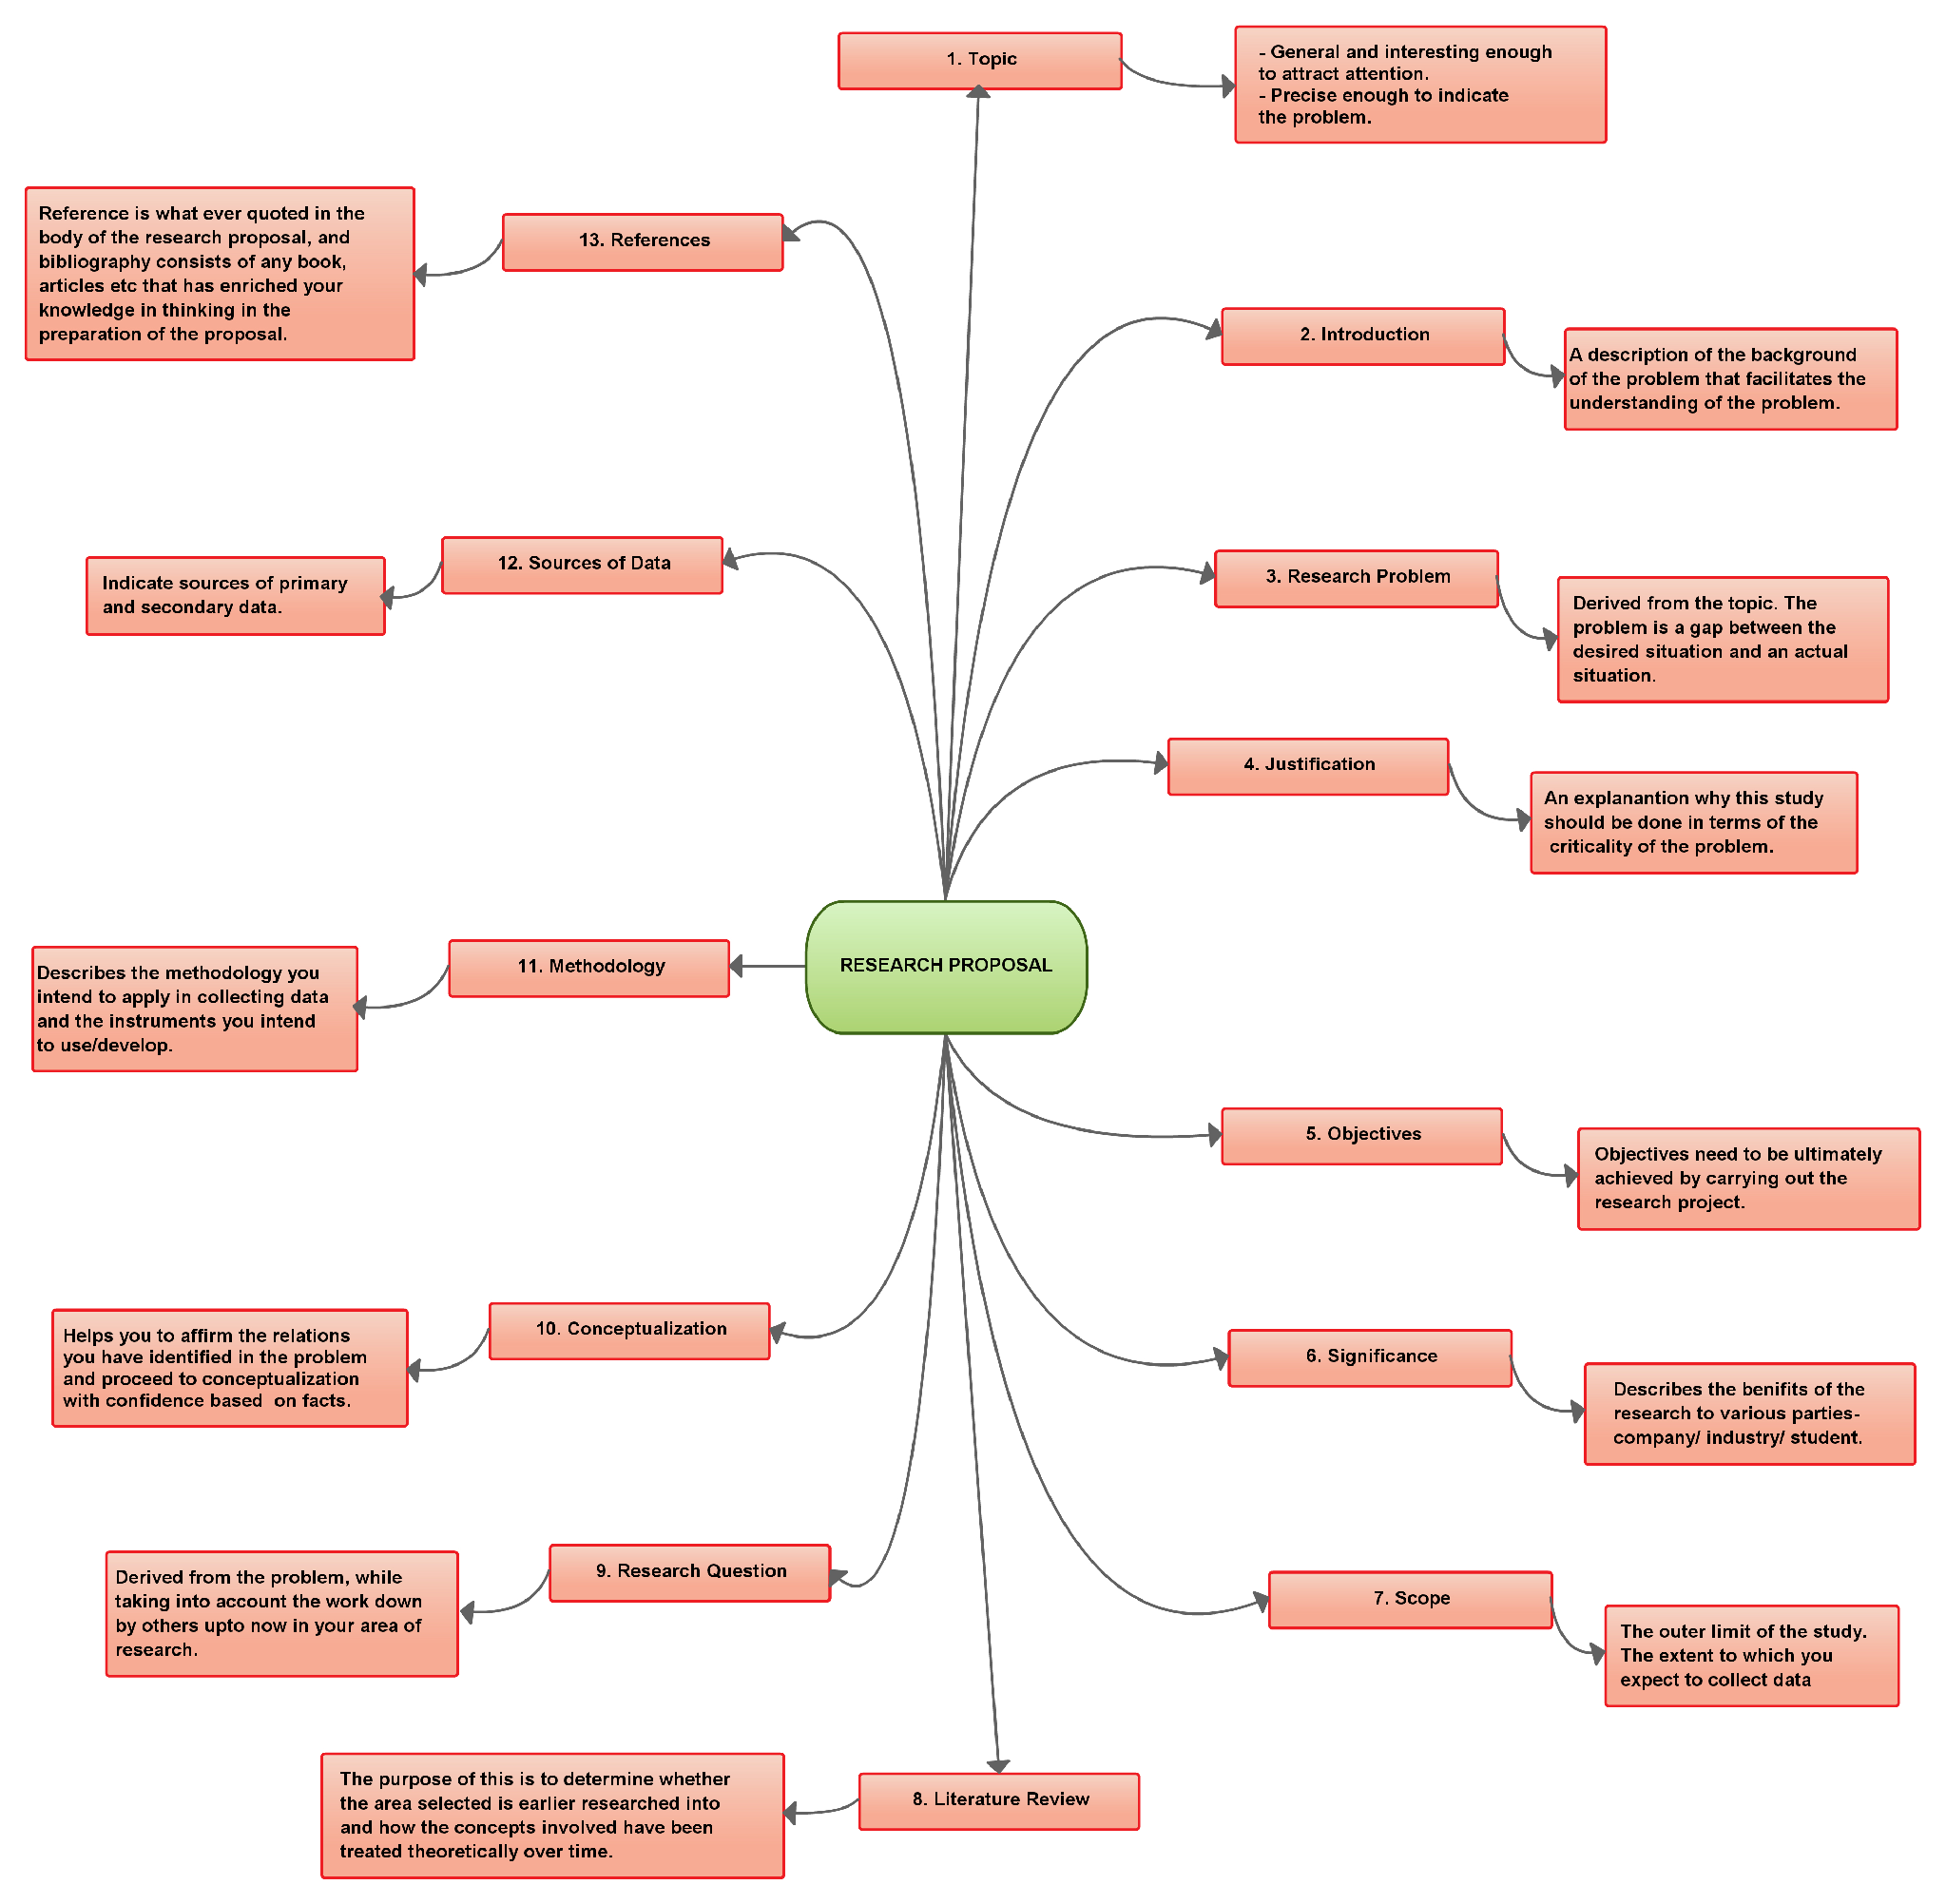
\includegraphics[scale=0.2]{fig/createlytest1.pdf}
\caption{This is a $\implies$ creately.com diagram}
\end{figure}

\begin{center}
\asyinclude{fig/comdiag.asy}
\end{center}

\begin{equation}\label{eq:star}
\xymatrix{
{\mathcal V}  \ar[r]^{S \quad\quad } \ar[d]_{\pi}
&  \mathsf{DynSys} \ar[d]^{U}  \\
 \op{(\et{\Graph})}  \ar[r]^{\quad\mathbb{P} }
&  \mathsf{Man} }
\end{equation}

Some text can be placed here \cite{Gould1994}

\begin{equation*}
\xy
(-18, 10)*+{\PP\lv T} ="1"; 
(18, 10)*+{\PP\rt T} ="2";
(-18,-10)*+{\PP\lv T'}="3";
(18,-10)*+{\PP \rt T'}="4";
{\ar@{->}^X "1";"2"};
{\ar@{->}^{\PP(\sigma|_{\lv T})} "3";"1"};
{\ar@{=}_{\PP(\sigma|_{\rt T}) = id } "4";"2"};
{\ar@{-->}_{\Ctrl(\sigma)X} "3";"4"};
\endxy
\end{equation*}


\section{Acknowledgements} 

DS supported by .
CRS .

%------bibliography---%
\bibliographystyle{unsrturl} 
\bibliography{ref/HO}
%---------------------%

\end{document}